\documentclass[12pt]{exam}
\newcommand{\hwnumber}{9}
\newcommand{\hwname}{String Buffers}
\newcommand{\duedate}{\formatdate{11}{11}{\YEAR} by \progDueTime} % day-month-year

\usepackage{../misc/latex/edition}  % Course semester
\usepackage{../misc/latex/c0}       % Listings style for c0
\usepackage{amsmath}
\usepackage{enumerate}
\usepackage[normalem]{ulem}
\usepackage{verbatim}
\usepackage[left=1in, right=1in, top=1in, bottom=1in]{geometry}
\usepackage{graphicx}
\usepackage{hyperref}
\usepackage{tikz}     \usetikzlibrary{shapes}
\usepackage{fancybox}
\usepackage[all]{xy}
\usepackage{wrapfig}
\usepackage{fancyvrb}
\usepackage{datetime}
\usepackage{etoolbox}
\usepackage{calc}
\usepackage[nomessages]{fp}
\usepackage{import}  % Like input and include, but respects subdirectories

\newcommand{\defaultQuestionLocation}{questions}
\newcommand{\inputQuestion}[2][\defaultQuestionLocation/]{%
  \subimport{#1}{#2}
}
% Subdirectories of \defaultQuestionLocation containing code and pictures
\newcommand{\code}{code}
\newcommand{\img}{img}


%%% ic: frontmatter macros
\newcommand{\specialInstructions}{}
\newcommand{\HWNUMBER}
{\ifdefempty{\hwnumber}{__}{%
  \ifnumless{\hwnumber}{10}{0\hwnumber}{\hwnumber}}}
\newcommand{\hwtype}{Written Homework}

%%% ic: 'exam' tweaks
\renewcommand{\half}{.5} % Half points

\newcommand{\Question}[2][]
 {\ifstrempty{#1}
    {\question{\bf #2}}
    {\question[#1]{\bf #2}}
  \immediate\write\rubricfile{}%
  \immediate\write\rubricfile{Question \thequestiontitle:}%
  \immediate\write\rubricfile{==========}
 }

%%% ic: Support for editable PDF
% counter name (some viewers misbehave if always the same)
\newcounter{editable}
\newcommand{\nextField}{\addtocounter{editable}{1}q\arabic{editable}}
\newcommand{\NextField}
 {\makebox[0pt][r]{\scalebox{0.1}{\color{White}\nextField}}}

% Color of edit area
\newcommand{\editAreaColor}{red}
% Single line answer:   \editableLine[extra parameters (optional)]{line width}
\newcommand{\editableLine}[2][]
{\textcolor{\editAreaColor}{%
 \underline{\hspace*{-0.25em}%
 \raisebox{-0.5ex}{%
 \TextField[width=#2, borderwidth=0, #1]{\NextField}}}}%
}
% Single line answer for code:  \editableLine[extra parameters (optional)]{line width}
\newcommand{\editableCodeLine}[2][]
{\textcolor{\editAreaColor}{%
 \underline{%
 \TextField[width=#2, height=1.5ex, borderwidth=0, #1]{\NextField}}}}
% Multiline answer:  \editableLine[extra parameters (optional)]{box height}
\newcommand{\editableBox}[2][]
{\leavevmode\hspace*{-0.1em}%
\TextField[height=#2, width=\linewidth,
           multiline=true, borderwidth=0.1, bordercolor=\editAreaColor,
           #1]{\NextField}}

%%%%% Same answer format as exams
\renewcommand{\rmdefault}{ppl}
\renewcommand{\sfdefault}{phv}
\newcommand{\answerColor}{Blue}

\ifprintanswers
\newcommand{\answer}[2]{\makebox[#1][c]{\color{\answerColor}#2}}
\else
\newcommand{\answer}[2]{\makebox[#1][c]{}\makebox[0pt]{\phantom{|}}}
\fi
\newcommand{\uanswer}[2]{\underline{\answer{#1}{#2}}}


%%% Write rubric snippet.  Usage:
% \RUBRIC
% any multi-line text (including \, #, %, whatever)
% ENDRUBRIC
%% (ENDRUBRIC should be on a line by itself)
\makeatletter
\def\RUBRIC
 {%
  \begingroup
  \let\do\@makeother\dospecials
  \endlinechar=`\^^J
  \@tofile%
 }
\def\ENDRUBRIC{ENDRUBRIC}
\def\@tofile#1^^J{%
  \def\@test{#1}%
  \ifx\@test\ENDRUBRIC
    \immediate\write\rubricfile{}  % End with an empty line
    \expandafter\@firstoftwo
  \else
    \expandafter\@secondoftwo
  \fi
  {\endgroup}%
  {\toks@{#1}%
   \begingroup\endlinechar=\m@ne
   \everyeof{\noexpand}%
   \xdef\@temp{\scantokens\expandafter{\the\toks@}}%
   \endgroup
   \immediate\write\rubricfile{\@temp}%
   \@tofile}%
}
\makeatother

%% Displays tags for an exercise in 'answer' mode
\newcommand{\TAGS}[1]
{\ifprintanswers%
  \rule{0em}{0ex}%
  \marginpar{\footnotesize%
    \fcolorbox{black}{Gray!25}{%
      \parbox[t]{2cm}{\raggedright\textbf{TAGS:}\\#1}}}%
  \ignorespaces%
 \fi}%


%% Page layout
\pagestyle{headandfoot}

\headrule
\header{\textbf{\courseNumber{} \hwtype{} \hwnumber}}
       {}
       {\textbf{Page \thepage\ of \numpages}}
\footrule
\footer{}{}{\COPYRIGHT}

\renewcommand{\partlabel}{\textbf{\thequestion.\thepartno}}
%\renewcommand{\partlabel}{\textbf{Task \thepartno}}
\renewcommand{\subpartlabel}{\textbf{\thesubpart.}}
\renewcommand{\thepartno}{\arabic{partno}}
\renewcommand{\thesubpart}{\alph{subpart}}
\pointpoints{pt}{pts}
\pointformat{\raisebox{0ex}[\height][0pt]{\fcolorbox{black}{yellow}{\themarginpoints}}}
\bonuspointformat{\raisebox{0ex}[\height][0pt]{\fcolorbox{black}{red}{\themarginpoints}}}
\marginpointname{\points}
\pointsinmargin
%\boxedpoints

\setlength\answerlinelength{2in}
\setlength\answerskip{0.3in}

\newcommand{\mkWrittenTitle}[1]{#1}
\newcommand{\mkDueDate}[1]{#1}
\newcommand{\mkEvalSummary}[1]{#1}
\newcommand{\mkGradetable}[1]{#1}



% This fixes an issue with the exam package version 2.6 and after,
% where 'framed' has been renamed to 'examframed' to avoid a conflict.
\ifcsmacro{examframed}{%
\newenvironment{framed}
{\begin{examframed}}
{\end{examframed}}
}{}

\begin{document}
\hwTitle

\noindent
In this programming assignment we will explore a useful data structure
for working with strings in an imperative language, a \emph{string
  buffer}. We'll write and test code for string buffers in both C0 and
C.

\bigskip
\noindent
The code handout for this assignment is at
\begin{center}
\whereisthetgz{strbuf-handout.tgz}
\end{center}
The file \lstinline'README.txt' in the code handout goes over the
contents of the handout and explains how to hand the assignment in.
There is a SEVEN (7) PENALTY-FREE HANDIN LIMIT.
Every additional handin will incur a small (5\%) penalty (even if
using a late day).

%% This assignment, like the DosLingos assignment, will treat superior
%% bug-finding in the files \lstinline'strbuf-test.c0' and
%% \lstinline'strbuf-test.c' as a bonus-worthy activity. Furthermore,
%% it will be necessary to have a reasonable set of test cases befure
%% course staff will be permitted to answer questions about code on
%% \qatool{} or in office hours.

\section{Strings in as Arrays of Characters}
\label{sec:cstrings}

C does not actually have a \lstinline'string' type. Instead, strings
are represented as arrays of characters. It is possible to represent
strings as arrays of characters in C0 as well.

The length of an array is not accessible outside of contracts in C0
and is not available at all in C, so one problem with representing
strings as arrays of characters is that we have to be able to tell
when the string stops! For this, we use the special ASCII value
\lstinline"'\0'", which has the numerical value 0 and is also called
the ``NUL terminator'' or the ``null character.'' This means that it
actually takes an array of length at least 9 to store a string, like
\lstinline'"Hi world"', that has length 8:
\begin{center}
  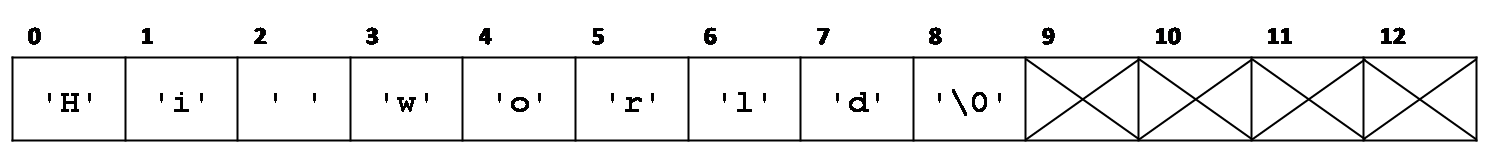
\includegraphics[width=\textwidth]{\img/str1.png}
\end{center}
The convention that we will adopt from C is to not count the NUL
terminator when we describe the length of this string.

Algorithms that deal with strings in C generally do not know the
length of the strings they are working with; instead, they just read
until the NUL terminator and then make sure not to read or write any
further. If the NUL terminator is missing, many of these algorithms
will keep right on reading or writing past the end of the array.


\subsection{String manipulation in C0 and C}

The built-in C0 \lstinline'string' library includes three functions
which may be useful. The function %
\lstinline'string_terminated(str, n)' %
checks that \lstinline'str[0..n)' contains a NUL-terminated
string. (Note that this string can have any length from $0$ to $n-1$
depending on where the NUL terminator is.) The function
\lstinline'string_from_chararray' constructs a C0 string from a
NUL-terminated character array, and the function
\lstinline'string_to_chararray' constructs a NUL-terminated character
array from a C0 string. This last function will be very helpful as you
are writing tests in C0. In C, string literals are treated as
\emph{constant arrays}, memory that you can read from but not write
to.  So both \lstinline|assert("Hello World"[6] == 'W')| and
\lstinline|assert("Hello World"[11] == 0)| are valid C assertions that
will pass.

In C, the library \lstinline[deletekeywords={string}]'string.h' can be
very useful in manipulating strings, and a translation of part of this
library into C0 is given in \lstinline'lib/cstring.c0' for use in your
code; you should make sure to look at and understand the functions in
this library. A reference for the complete C version of this library
is available at \url{http://www.cplusplus.com/reference/cstring/}.
You can also find more information in the Unix manual pages,
accessible with the command \lstinline'man'. For example, type %
\lstinline'man strcpy' %
into the Unix shell. You should familiarize yourself with these
functions to avoid duplicating their functionality in your code. This
would be considered bad style and is a possible source of
bugs. However, here are some common pitfalls of some library
functions:
\begin{itemize}
\item%
  Be aware of the runtimes, especially for \lstinline'strcat' and
  \lstinline'strncat'.
\item%
  As mentioned previously, \lstinline'strlen' does not consider the
  NUL terminator.
\item%
  Using \lstinline'strcpy' may access an array out of bounds if the
  source string is longer than the destination array.
\item%
  Using \lstinline'strncpy' does not guarantee that \lstinline'dest'
  will be NUL terminated if a NUL byte is not copied from the first
  \lstinline'n' bytes of \lstinline'src'.
\end{itemize}

For this library and its C0 translation to really make sense, it helps
to think of a C string as the combination of a C0 array and an
\emph{offset} describing where the string starts in the array. This
strategy lets us store multiple strings in the same array and even
save space by having strings overlap:
\begin{center}
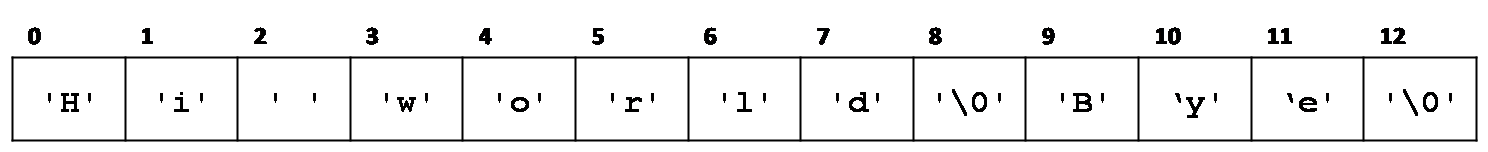
\includegraphics[width=\textwidth]{\img/str2.png}
\end{center}
If the array above is \lstinline'str', then we could say that
\lstinline'str+0' points to the string \lstinline'"Hi world"', that
\lstinline'str+3' points to the string \lstinline'"world"', that
\lstinline'str+9' points to the string \lstinline'"Bye"', and that
both \lstinline'str+8' and \lstinline'str+12' point to the empty
string. In C0 this syntax is not allowed, so
\lstinline'lib/cstring.c0' takes two arguments per string --- the base
array and the offset. In C, \emph{pointer arithmetic} and the
conflation of pointers and arrays will allow us to actually add
positive integers to pointers and get occasionally meaningful results:
\begin{quote}
\begin{lstlisting}
// In C
char *str1 = "Hi world";
assert(0 == strcmp("world", str1 + 3));
\end{lstlisting}
\end{quote}
Therefore the \lstinline[deletekeywords={string}]'string.h' library
only has to take one \lstinline'char*' argument per string. Pointer
arithmetic like this is often a bad idea, but it's important to be
aware of it.


\section{String Buffers: Overview}
\label{sec:overview}

In practice, manipulation of strings as mutable arrays is tedious and
error-prone, which is one of the reasons that string buffers are
useful.  A \emph{string buffer} is fundamentally an adaptation of an
unbounded array.  When we allocate a string buffer, we allocate an
array of a given initial size, but leave it empty.  This is the
initial state of a string buffer \lstinline'sb' allocated with size
13:
\begin{center}
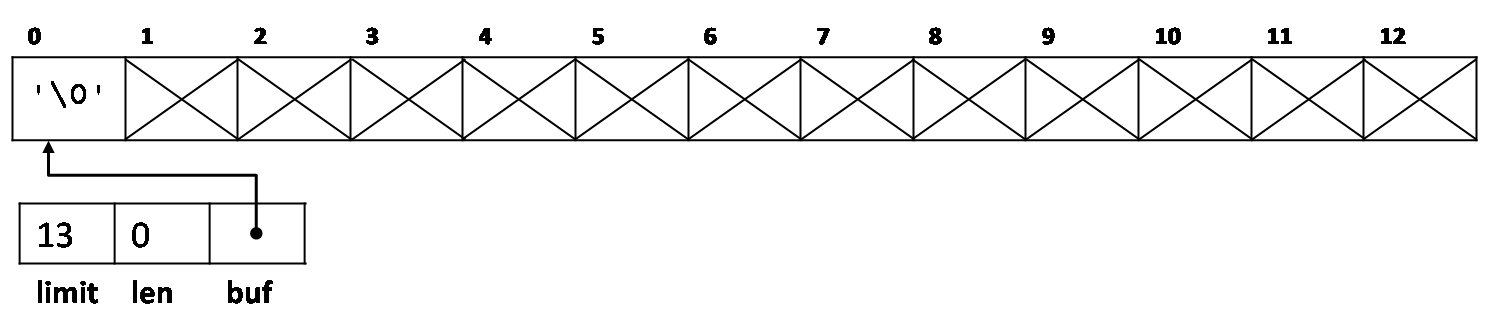
\includegraphics[width=\textwidth]{\img/strbuf0.png}
\end{center}
Then we repeatedly add strings to the end of the buffer.  For example,
if we add the string \lstinline'"over"' to \lstinline'sb', we get this
picture:
\begin{center}
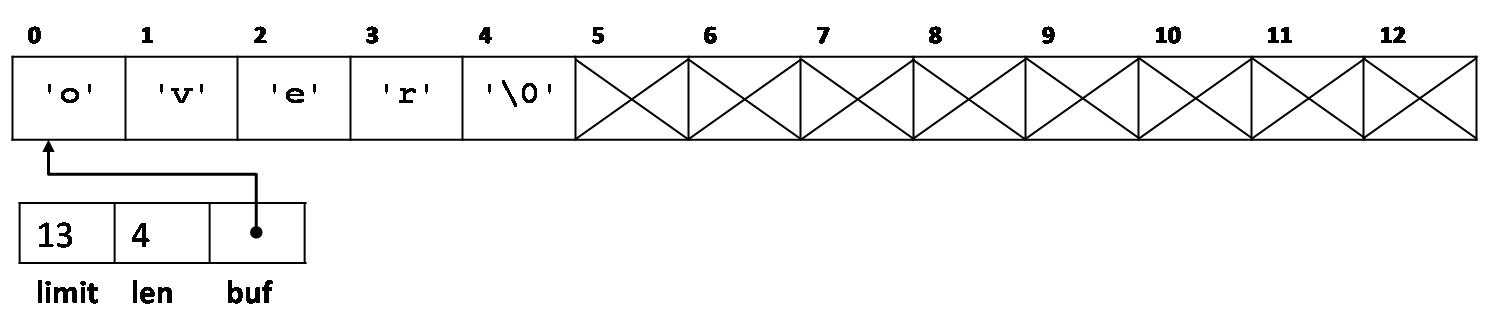
\includegraphics[width=\textwidth]{\img/strbuf1.png}
\end{center}
If we next add the string \lstinline'"loading"' to the buffer, we
get this picture:
\begin{center}
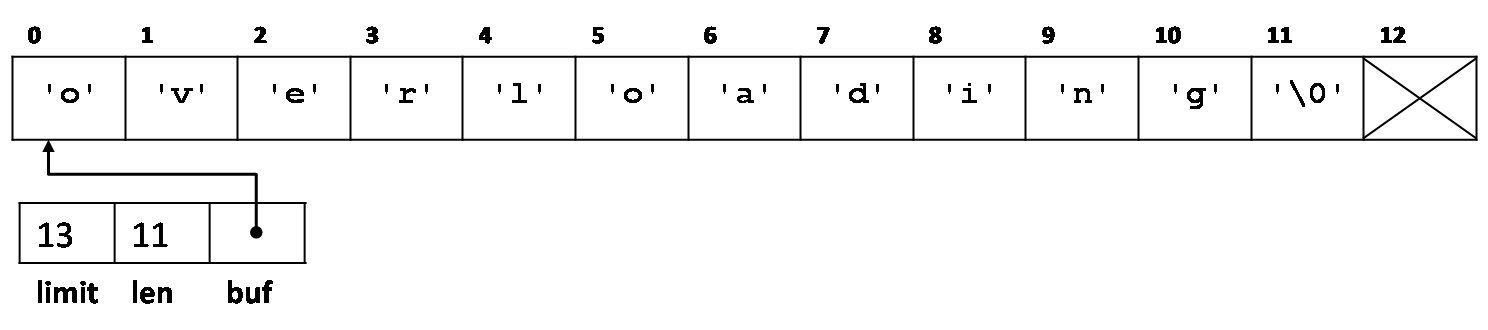
\includegraphics[width=\textwidth]{\img/strbuf2.png}
\end{center}
The corresponding C calls, with the functions explained later in this
writeup, are:
\begin{lstlisting}
  struct strbuf *sb = strbuf_new(13);
  strbuf_add(sb, "over", 4);     // In C0 use string_to_chararray("over")
  strbuf_add(sb, "loading", 7);  // ...same thing here.
\end{lstlisting}
When we run out of space in the current buffer, we resize it by
allocating a larger array and copy the current elements to the new
array.  The size increase has to be sufficient to guarantee a
worst-case amortized time of $O(k)$ to add a string of length $k$ to
the buffer.

Unlike most of the other data structures we have considered in 15-122,
we will expose the representation of our string buffers to clients of
our library.  One benefit of this approach is that it allows the
client to directly access the fields of a string buffer, avoiding a
proliferation of interface functions.  One disadvantage is that this
approach locks us into a particular representation.  Furthermore, the
client is partially responsible for maintaining the data structure
invariants, and we have to be very careful about those invariants. For
example, the client can write to index \lstinline'12' in the buffers
above without violating the data structure invariants, so we must
treat the unspecified contents of the array as really unspecified.


\section{String Buffers in C0}

The C0 type \lstinline'struct strbuf' of string buffers is declared as
follows:

\begin{quote}
\begin{lstlisting}
struct strbuf {
  int limit;
  int len;
  char[] buf;
};
\end{lstlisting}
\end{quote}
A string buffer \lstinline'sb', a pointer to a %
\lstinline'struct strbuf', %
must satisfy the following properties:
\begin{enumerate}
\item%
  The buffer \lstinline'sb' must not be \lstinline'NULL'.
\item%
  The number of characters allocated in \lstinline'buf' (the size of
  the array) must be equal to \lstinline'limit'.
\item%
  The segment \lstinline'buf[0..len]' is a valid NUL-terminated string
  of length \lstinline'len'.  This means all the characters in
  \lstinline'buf[0..len)' must be non-NUL (\lstinline"'\0'"), and
  \lstinline'buf[len]' must be NUL.
\end{enumerate}
Note that these invariants do \emph{not} say anything about the
unspecified portion of the array after the NUL terminator. Your data
structure invariants should not either.

\begin{task}[4]
\TAGS{array, ds-invariant, string}
  In the file \lstinline'strbuf.c0', write the function
\begin{quote}
\begin{lstlisting}
bool is_strbuf(struct strbuf* sb);
\end{lstlisting}
\end{quote}
to check that \lstinline'sb' is a pointer to a valid string buffer. It
should return \lstinline'false' rather than failing a contract
whenever possible.
\end{task}

Allocation for a string buffer is straightforward: the buffer
initially contains the empty string and the initial size for
\lstinline'buf' is supplied by the client. We will also write a
function \lstinline'strbuf_str', which should return a fresh copy of
the string-occupied part of the string buffer. This returned array
should be NUL-terminated and no longer than necessary.

\begin{task}[3]
\TAGS{array, ds-invariant, string}
  In the file \lstinline'strbuf.c0', write the functions
\begin{quote}
\begin{lstlisting}
struct strbuf* strbuf_new(int initial_limit); // *Strictly* positive
char[] strbuf_str(struct strbuf* str);
\end{lstlisting}
\end{quote}
according to the description above.
\end{task}

\subsection{Adding a String}
\label{sec:add}

We can read or write to individual characters at index \lstinline'i'
in the string buffer \lstinline'sb' simply with
\lstinline'sb->buf[i]'.  To add a string to a string buffer we
concatenate it at the end of the string already in the buffer when
there is enough space.  Of course, we must do this in such a way that
all invariants of the string buffer data structure are preserved.
When there is not enough room we need to allocate more space so that
the result fits into the array. However, you must not allocate a new
array unless it is \emph{necessary}: resizing is not allowed whenever
the added string fits in the array! Your implementation should exploit ideas
from our implementation of unbounded arrays to make sure adding a
string of length $k$ takes amortized time in $O(k)$.

\begin{task}[5]
\TAGS{amortized-cost, array, ds-invariant, string}
  In the file \lstinline'strbuf.c0', implement functions
\begin{quote}
\begin{lstlisting}
void strbuf_add(struct strbuf* sb, char[] str, int str_len);
void strbuf_addstr(struct strbuf* sb, char[] str);
\end{lstlisting}
\end{quote}
The first form can be used if the length \lstinline'str_len' of the
string \lstinline'str' is known. It should be a precondition of
\lstinline'strbuf_add' that \lstinline'str_len' is the length of the
string stored in \lstinline'str'. (The length of the string,
\underline{not} the length of the array.)

The second function can be used if that information is not readily
available. You should take into account their similarity to simplify
your code: \lstinline'strbuf_addstr' should be a one-liner.
\end{task}

\paragraph{Important:}
It may be very tempting to use the
\lstinline[deletekeywords={string}]'string.h' functions
\lstinline'strcat' or \lstinline'strncat' (implemented in
\lstinline'lib/cstring.c0') when writing these functions. However,
this will fail to achieve the required $O(k)$ runtime. We're told in
\lstinline'man strcat':
\begin{lstlisting}
// A simple [C] implementation of strncat() might be:

char *strncat(char *dest, const char *src, size_t n) {
  size_t dest_len = strlen(dest);
  size_t i;
  for (i = 0 ; i < n && src[i] != '\0' ; i++) {
    dest[dest_len + i] = src[i];
  }
  dest[dest_len + i] = '\0';
  return dest;
}
\end{lstlisting}
The key is that there is a call to \lstinline'strlen', which runs in
$O(len)$. Therefore, any solution using \lstinline'strcat' or
\lstinline'strncat' would run in $O(len + k)$ time, which is not
acceptable.

\subsection{Unit Testing}

We will run your tests both against your own code, correct
implementations of string buffers in C0, and buggy implementations of
string buffers in C0. You should write tests that will fail for as
many buggy implementations as possible.

For these test cases, we're asking you to do something a little bit
new: your test cases need to pass for \emph{any} correct
implementation of string buffers.  One example: it is a requirement
that \lstinline'strbuf_add' and \lstinline'strbuf_addstr' only
allocate a larger buffer when they are absolutely required to, but the
specific amount that the buffer grows by is up to the
implementation. Therefore, don't submit unit tests that try to check
the specific new size of the post-increase buffer, or the autograder
will complain that these tests fail on correct implementations. Your
unit tests can check that the buffer doesn't resize until absolutely
required, as this behavior is required for any correct
\lstinline'strbuf_add' or \lstinline'strbuf_addstr' implementation.

Your tests should use the \lstinline'assert()' function instead of
using contracts so that the unit tests run whether or not you are
compiling with \lstinline'-d'.

\begin{task}[4]
\TAGS{testing}
  Write and submit test cases in \lstinline'strbuf-test.c0' that test
  your C0 implementation of string buffers.
\end{task}

To get these points, your test cases must catch an
implementation that is correct except for a specific bug in Task 1, a
second implementation that is correct except for a specific bug in
Task 2, and a third implementation that is correct except for a
specific bug in Task 3.


\subsection{Advice}

All your functions should be relatively short.  The difficulty is to
reason properly about invariants, string lengths, allocation sizes,
and effects of various operations to get it \emph{exactly} right.  We
will test your code thoroughly, in at least the following respects:
\begin{enumerate}
\item%
  The strength of your contracts, specifically, the preconditions and
  data structure invariants.
\item%
  The correctness of the answers.
\item%
  Amortized running time and memory usage.
\item%
  Memory footprint (including allocating more memory than you need).
\end{enumerate}


\section{String buffers in C}

For the last part of the assignment, we will turn our C0 string
buffers into C string buffers. In C, it is \emph{not possible} to
check the length of an array, so it will no longer be possible to
enforce certain invariants of your data structure.

\subsection{Adapting C0 code to C}

Your \lstinline'strbuf.c' should begin with at least the following declarations:

\begin{quote}
\begin{lstlisting}[deletekeywords={string}]
#include <stdlib.h>        // Standard C library: free(), NULL...
#include <stdbool.h>       // Standard true, false, and bool type
#include <string.h>        // Standard C version of lib/cstring.c0
#include "lib/contracts.h" // Our contracts library
#include "lib/xalloc.h"    // Our allocation library
#include "strbuf.h"        // The string buffer interface
\end{lstlisting}
\end{quote}

Here is an \emph{incomplete} list of the changes you will need to make
as you adapt your C0 string buffers to C:
\begin{itemize}
\item%
  Change array types like \lstinline'char[]' to pointers
  \lstinline'char*'. Be careful: this means that you now have to check
  that arrays are non-NULL in your code and data structure invariants!
\item%
  Modify uses of the \lstinline'lib/cstring.c0' library to be uses of
  the standard \lstinline[deletekeywords={string}]'string.h' library.
\item%
  Change calls from \lstinline'alloc' and \lstinline'alloc_array'
  to their C analogues. We strongly recommend the use of the (local)
  \lstinline'xalloc' library which defines \lstinline'xmalloc' and
  \lstinline'xcalloc'. These functions abort rather than returning
  \lstinline'NULL' when no more memory is available.
\item%
  Change \lstinline'//@requires', \lstinline'//@ensures', and
  \lstinline'//@assert' C0 contracts into \lstinline'REQUIRES()',
  \lstinline'ENSURES()', and \lstinline'ASSERT()' C contracts.
\item%
  The string buffer is responsible for managing its character
  array, so when \lstinline'strbuf_add' or \lstinline'strbuf_addstr' need to
  increase the size of that array, it's necessary for the functions to
  make sure that the old array gets freed. \emph{Your test cases
    should free all allocated memory.}
\item%
  Adapt to the use of \lstinline'size_t' instead of \lstinline'int' for
  quantities that are supposed to be array offsets. The type
  \lstinline'size_t' is unsigned, so you don't need to check that they're
  greater than zero.
\end{itemize}
As a stylistic issue, we write
\begin{quote}
\begin{lstlisting}
int* x = alloc(int);
char[] A = alloc_array(char, 10);
\end{lstlisting}
\end{quote}
in C0 but write
\begin{quote}
\begin{lstlisting}
int *x = xmalloc(sizeof(int));
char *A = xcalloc(10, sizeof(char));
\end{lstlisting}
\end{quote}
in C. Attaching the \lstinline'*' to the variable instead of the type
is consistent with the C idea of making the definition of a variable
look like the way it is used. We won't be picky about this stylistic
issue on this assignment, though.

\begin{task}[5]
\TAGS{c-array, c-memory, string}
  Copy the implementation of \lstinline'strbuf.c0' to
  \lstinline'strbuf.c', making sure to include the interface by
  writing \lstinline'#include "strbuf.h"' within this file.
\end{task}

A word of warning: our tests for \lstinline'strbuf.c' are not exactly
the same as our tests for \lstinline'strbuf.c0', and it's possible
that things that we missed with earlier testing will be caught by the
C tests!

\subsection{Handling Deallocation}

As is common with C0 to C translations, we have to write a function
that deallocates the memory reserved for our data structure. Rather
than having the deallocation function free both the %
\lstinline'struct strbuf' %
and the buffer \lstinline'buf', we will return the embedded
\lstinline'buf' array without freeing it and pass ownership of it to
the client, who becomes responsible for (eventually) freeing it.  This
allows us to detach the current contents of the string buffer without
making a copy.

\begin{task}[2]
\TAGS{c-array, c-memory, string}
  In the file \lstinline'strbuf.c', implement the function
\begin{quote}
\begin{lstlisting}
char *strbuf_dealloc(struct strbuf *sb);
\end{lstlisting}
\end{quote}
  according to the description above.
\end{task}

\subsection{Unit Testing}

Your C unit tests should again use \lstinline'assert()' rather than
contracts.  To use the \lstinline'assert()' function in C, you need to
\lstinline[deletekeywords={assert}]'#include <assert.h>'.  In addition
to running your tests, you should use the \lstinline'valgrind' tool to
check for invalid memory access and memory leaks. When you compile
with the \lstinline'-g' flag, \lstinline'valgrind' can give you
valuable information about where undefined behavior and memory leaks
are occurring.

For your C0 tests, you can create C-style strings easily with
\lstinline'string_to_chararray'. In C, there are several ways to
declare a string.

\begin{enumerate}
\item%
  On the heap with \lstinline'xmalloc' and \lstinline'xcalloc', the
  same way that you would allocate an array of any other type:
\begin{quote}
\begin{lstlisting}
size_t len = 10;
char *s0 = xmalloc(len * sizeof(char));
char *s1 = xcalloc(len, sizeof(char));
\end{lstlisting}
\end{quote}
\item%
  On the program stack. C lets you declare and initialize arrays on
  the stack that are automatically freed when the function
  returns. One way of initializing such stack-allocated arrays is to
  write a string.
\begin{quote}
\begin{lstlisting}
char s[] = "C is fun.";
\end{lstlisting}
\end{quote}
\item%
  String literals. These strings are stored in read-only memory; you
  can't write to them.
\begin{quote}
\begin{lstlisting}
const char *s = "C is scary.";
\end{lstlisting}
\end{quote}
  The \lstinline'const' keyword isn't required, but the compiler may catch
  attempts to modify the string, instead of causing undefined behavior
  at runtime.
\end{enumerate}
A trick for creating a string on the heap from the contents of a
string literal, which may help in your testing code, is to use
\lstinline"strcpy":
\begin{lstlisting}
  const char *s_lit = "Hello World!";
  char *s_heap = xmalloc((strlen(s_lit) + 1) * sizeof(char));
  strcpy(s_heap, s_lit);
\end{lstlisting}

\begin{task}[2]
\TAGS{testing}
  Write and submit test cases in \lstinline'strbuf-test.c' that test
  your C implementation of string buffers.
\end{task}

\end{document}








\subsection{The NUL Terminator}
A common source of confusion when working with strings in general with
C (and especially true on this assignment) is managing the NUL
terminator. The NUL terminator essentially signifies the end of the
string. It has an ASCII value of 0 and is represented as the character
\lstinline"'\0'". Many string library functions, such as
\lstinline'strlen' rely on the NUL terminator; calling them when the
NUL terminator is missing
leads to undefined behavior.

Since the NUL terminator is a character itself, you need to ensure
that there is sufficient memory to store it. For example, if I want to
store ``cat'' in a string, 4 bytes are needed: 3 for the contents of
the string and 1 for the NUL terminator. This is reflected in the
diagrams shown in Section~\ref{sec:overview}. Therefore, you need to
take this into consideration when allocating heap memory. Note that
\lstinline'strlen' does not include the NUL terminator in its
result. There are some situations when this behavior is desirable, but
others where you must add one to the result. If you observe invalid
memory accesses using \lstinline'valgrind', mishandling the NUL
terminator is a common cause.

Strings that are created from double-quotes automatically include the
NUL terminator, so you don't need to worry about those cases. To
illustrate these points, consider this code:
\begin{lstlisting}
int main () {
  char s[] = "Hello World!";
  printf("strlen: %zu sizeof: %zu\n", strlen(s), sizeof(s));
  return 0;
}
\end{lstlisting}
When run, this code prints \lstinline'strlen: 12 sizeof: 13'. Recall
that \lstinline'sizeof' behaves differently with stack arrays compared
to heap arrays.


\subsection{Standard \lstinline'string.h' Functions}

You will find it helpful to use some \lstinline'string.h' library
functions when writing your code. A reference is available at
\url{http://www.cplusplus.com/reference/cstring/}. You can also find
more information in the unix man pages. For example, type
\lstinline'man strcpy' into the unix shell. You should familiarize
yourself with these functions to avoid duplicating their functionality
in your code. This would be considered bad style and a possible source
of bugs. However, here are some common pitfalls of some library
functions:
\begin{itemize}
\item%
  Be aware of the runtimes. An example using \lstinline'strncat' is
  given in Section~\ref{sec:add}. In some cases, the man pages provide
  a sample simple implementation.
\item%
  As mentioned previously, \lstinline'strlen' does not include the NUL
  terminator.
\item%
  Using \lstinline'strcpy' may continue past the end of an array if
  \lstinline'src' is longer than \lstinline'dest'.
\item%
  Using \lstinline'strncpy' does not guarantee that \lstinline'dest'
  will be NUL terminated if a NUL byte is not copied from the first
  \lstinline'n' bytes of \lstinline'src'.
\end{itemize}

\noindent
\textbf{\large{Assignment: String Buffers (25 points in total)}}
\vspace{1em}

\paragraph{Starter code.}
Download the file \lstinline'hw7-handout.tgz' from the course website.
When you untar it, you will find \lstinline'strbuf.h' (the header file
for the string buffer library for you to write), a
\lstinline'Makefile', and a \lstinline'lib/' directory with some
provided libraries.  You should not modify or hand in any of the given
files.  Instead, you should write \lstinline'strbuf.c' and
\lstinline'strbuf-test.c'.

\paragraph{Compiling and running.}
You will compile and run your code using the standard \lstinline'gcc'
compiler.  We have provided you with a \lstinline'Makefile' that can
save you from typing lengthy shell commands.  You are not responsible
for understanding the make file, but we invite you to read it anyway,
since it is a common tool for C and Unix.  You should compile and run
with
\begin{lstlisting}
  % make strbuf-d  # Contracts checked.
  % ./strbuf-d
  % make strbuf    # Contracts not checked.
  % ./strbuf
\end{lstlisting}

\paragraph{Submitting.}
Once you've completed some files, you can submit them to
Autolab. There are two ways to do this:

From the terminal on Andrew Linux (via cluster or ssh) type:
\begin{lstlisting}
 % handin hw7 strbuf.c strbuf-test.c
\end{lstlisting}
Your score will then be available on the Autolab website.

Your files can also be submitted to the web interface of Autolab.  To
do so, please \lstinline'tar' them, for example:
\begin{lstlisting}
 % tar -czvf sol.tgz strbuf.c strbuf-test.c
\end{lstlisting}

Then, go to \url{https://autolab.cs.cmu.edu/15122-m13} and submit them
as your solution to homework 7 (\hwname).

You may submit your assignment up to 25 times.  When we grade your
assignment, we will consider the most recent version submitted before
the due date.

\paragraph{Annotations.}
Be sure to include appropriate \lstinline"REQUIRES",
\lstinline"ENSURES", and \lstinline"ASSERT" macros in your program.
If you write any auxiliary functions, include precise and appropriate
pre- and postconditions.

You should write these as you are writing the code rather than after
you're done: documenting your code as you go along will help you
reason about what it should be doing, and thus help you write code
that is both clearer and more correct. \textbf{Annotations are part of
  your score for the programming problems; you will not receive
  maximum credit if your annotations are weak or missing.}

\paragraph{Unit testing.}
You should write unit tests for your code.  We recommend writing these
early to check your code as you move forward.  See
Section~\ref{sec:test}.

\paragraph{Style.}
Strive to write code with \emph{good style}: indent every line of a
block to the same level, use descriptive variable names, keep lines to
80 characters or fewer, document your code with comments, etc.  If you
find yourself writing the same code over and over, or find functions
becoming very long, you should write a separate function to handle
that computation and call it whenever you need it.  We will read your
code when we grade it, and good style is sure to earn our good graces.
Feel free to ask on \qatool{} if you're unsure of what constitutes good
style. You may also find it helpful to refer to the course style guide
at
\url{http://www.cs.cmu.edu/~rjsimmon/15122-s13/rec/style_guide.pdf}.

\setcounter{task}{-1}
\begin{task}
  As with the previous few assignments, we expect you to be writing
  code with good style; we have given you feedback on style for
  multiple assignments and we have shown you many examples of code
  with reasonable style.  This assignment will initially have all 25
  points assigned through the autograder, but up to 5 points may be
  deducted for style issues.
\end{task}


\newpage
\section{String Buffer Representation}
\label{sec:strbuf-invs}

The interface to string buffers is different from many of our prior
examples because we do not keep the representation abstract.  Instead,
we announce the precise form of the internal representation.  One
advantage is that this allows the client to directly access the fields
of a string buffer, avoiding a proliferation of interface functions.
A disadvantage is that now the client is partially responsible for
maintaining the data structure invariants.  Moreover, we lock
ourselves into a particular representation.  In this particular case,
however, it seems the advantages of a concrete representation may
outweigh its disadvantages.

We have in the file \lstinline'strbuf.h':
\begin{lstlisting}
struct strbuf {
  size_t alloc;    /* alloc > 0, bytes allocated for buf */
  size_t len;      /* len < alloc */
  char *buf;       /* buf != NULL, buf[len] == '\0', strlen(buf) == len */
};
bool is_strbuf(struct strbuf *sb);
\end{lstlisting}
Because the client can see the implementation, we also publish the
interface to the \lstinline'is_strbuf' function.

A string buffer must satisfy the following properties:
\begin{enumerate}
\item%
  \lstinline'buf' is not \lstinline'NULL'
\item%
  The number of characters allocated in \lstinline'buf' must be equal
  to \lstinline'alloc'.  Note that this cannot be checked dynamically,
  when the code executes.
\item%
  The segment \lstinline'buf[0..len]' is a valid C string of length
  \lstinline'len'.  This means all the characters in
  \lstinline'buf[0..len)' must be non-\lstinline'NUL'
  (\lstinline"'\0'"), and \lstinline'buf[len]' must be
  \lstinline'NUL'.
\end{enumerate}

\begin{task}[6]
  In a file \lstinline'strbuf.c', write the function
\begin{lstlisting}
  bool is_strbuf(struct strbuf *sb);
\end{lstlisting}
  to check that \lstinline'sb' is a pointer to a valid string buffer
  (to the extent that this is possible in C).  Make sure you
  \lstinline'#include' all appropriate library headers (\lstinline'.h'
  files), including \lstinline'strbuf.h'.
\end{task}

\section{Allocation and Deallocation}
\label{sec:alloc}

Allocation of a string buffer is straightforward, given what we
have said above.  An initial allocation size for \lstinline'buf' is
supplied by the client.
\begin{lstlisting}
  struct strbuf *strbuf_new(size_t alloc_init);
\end{lstlisting}

Deallocation is a little bit trickier.  Throughout the lifetime of a
string buffer, \emph{it always owns the \lstinline'buf' array}.  It is
essential that you understand this invariant.  It is necessary so that
the string buffer implementation can resize the \lstinline'buf' array
as needed; it could not do so if it didn't own the array.

When we deallocate the string buffer, we return the embedded
\lstinline'buf' array and pass ownership of it to the client, who
becomes responsible for (eventually) freeing it.  This allows us to
detach the current contents of the string buffer without making a
copy.

\begin{lstlisting}
  char *strbuf_dealloc(struct strbuf *sb);
\end{lstlisting}

Also, at any time the client can ask for a string that's a copy of the
one currently in the string buffer.  This copy should only occupy the
exact memory needed, and may be much shorter than the buffer itself.
The client also obtains ownership of this string and will eventually
be responsible for freeing it.

\begin{lstlisting}
  char *strbuf_str(struct strbuf *sb);
\end{lstlisting}

\begin{task}[7]
  Inside the file \lstinline'strbuf.c', implement functions
  \lstinline'strbuf_new', \lstinline'strbuf_dealloc', and
  \lstinline'strbuf_str' according to the description above.
\end{task}


\section{Contracts}
\label{sec:contracts}

Your functions should have contracts on them that are as precise as is
possible in C\@.  We have already discussed the string buffer data
structure invariants in Section~\ref{sec:strbuf-invs}.

Since we cannot properly check the length of arrays, you should assume
that arguments of type \lstinline'char*' are either \lstinline'NULL'
or valid C strings.  This means they are allocated somewhere in memory
(heap, stack, or data segment) and they are properly terminated by the
\lstinline'NUL' character \lstinline"'\0'".

If a function receives a string \lstinline's' and its purported length
\lstinline'len', your precondition should check that
\lstinline'strlen(s) == len' (after ascertaining that \lstinline's' is
not \lstinline'NULL').  Similarly, if a function returns a string of
known length, your postcondition should check the length.

When we test your code, we may supply \lstinline'NULL' for any
pointers to make sure appropriate contract exceptions are raised, but
any strings we apply it to will be properly terminated by
\lstinline"'\0'".

\section{Test Cases}
\label{sec:test}

This time, we require you to write and hand in test cases.  To
simplify matters, we only request a single file \lstinline'strbuf-test.c'
defining a function \lstinline'main()' that does black-box testing of the
string buffer implementation, using only what is exposed in the
interface in file \lstinline'strbuf.h'.  Tests should have the form of
\lstinline'assert()' statements that verify the correctness of the
implementation on correct input. \textbf{Note:} use ``hard asserts'',
i.e. \lstinline'assert()',
not \lstinline'ASSERT'.

\begin{task}[6]
  In the file \lstinline'strbuf-test.c', write test cases that are
  exercised when the function \lstinline'main()' is called.

  Your test should not pass inputs to the function that would violate
  the function's preconditions, or modify the data representation in
  ways that's inconsistent with the invariants.
\end{task}

We will link your testing code with various plausibly faulty
implementations to verify reasonable coverage, using the black-box
testing techniques we discussed in lecture.

You should revisit the specification for each of the above tasks and
determine how to write a test that would catch an implementation that
does not follow the specification. Be sure to consider not only the
contents of the string buffer, but also memory, e.g. when new memory
should and shouldn't be allocated. Naturally, incorrect memory
management that cannot be checked by your code will \textbf{not} be
tested.

You may find it helpful to refer back to your twitterlab code as a
reminder of how to structure your tests. Similar to that assignment,
you do not need to identify all bugs to receive full credit.

To help you with this task, you will be able to try to catch some of
the bugs without submitting to Autolab. However, the remaining bugs
are only accessible by submitting to Autolab. See README.txt for
details.

\end{document}
